\documentclass{beamer}
\usepackage[utf8]{inputenc}
\usetheme{PaloAlto}
\usecolortheme{default}
\usepackage{tikz}
\usetikzlibrary{shapes,arrows,chains}

\title[Métodos de Segmentação Automática de Sinais de sEMG]{Métodos de Segmentação Automática de Sinais de Eletromiografia de Superfície}
\subtitle{para Classificação de Movimentos Utilizando RNA}
\author[Cunha] {Vicente Cunha \\ \and Alexandre Balbinot (orientador)}
\institute[UFRGS]{Universidade Federal do Rio Grande do Sul}
\date[dezembro de 2015]{Porto Alegre, dezembro de 2015}
\subject{Biomedical Science}

\begin{document}
	
	\frame{\titlepage}
	
	\begin{frame}
		\frametitle{Sumário}
		\tableofcontents[]
	\end{frame}
	
	\section[Introdução]{Introdução}
	
	\begin{frame}
		\frametitle{Eletromiografia}
		\framesubtitle{Principais aplicações}
		\begin{columns}[c]
			\column{.5\textwidth}
				\begin{figure}
					Diagnóstico de desordens neuromusculares
					\begin{center}
						\includegraphics[width=\textwidth]{./img/disorders.png}
					\end{center}
				\end{figure}
				
			\column{.5\textwidth}
				\begin{figure}
					Atuação de Próteses Mioelétricas
					\begin{center}
						\includegraphics[width=\textwidth]{./img/prosthesis.jpg}
					\end{center}
				\end{figure}
		\end{columns}
	\end{frame}

	\begin{frame}
		\frametitle{NinaPro}
		\framesubtitle{\emph{Non-Invasive Adaptive Hand Prosthetics} - IDIAP \emph{Research Institute 2012}}
		
		\begin{columns}[c]
			\column{.5\textwidth}
				\begin{figure}
					\begin{center}
						\includegraphics[width=\textwidth]{./img/classificationExample.jpg}
					\end{center}
				\end{figure}
				\column{.5\textwidth}
				\begin{alertblock}{Etapas Necessárias para a Classificação de Movimentos}
				\begin{itemize}
					\item Segmentação do Sinal em Trechos de Interesse
					\item Extração de Características dos Segmentos
					\item Treinamento de RNA
				\end{itemize}
			\end{alertblock}
		\end{columns}

		\begin{block}{Objetivos deste Trabalho}
			Proposição e implementação de métodos de segmentação automática e consequente classificação de movimentos utilizando RNA.
		\end{block}

	\end{frame}

%	\begin{frame}
%		\frametitle{Objetivos do Trabalho}
%		
%		\begin{alertblock}{Etapas Necessárias para a Classificação de Movimentos}
%		\begin{itemize}
%			\item Segmentação do Sinal em Trechos de Interesse
%			\item Extração de Características dos Segmentos
%			\item Treinamento de RNA
%		\end{itemize}
%		\end{alertblock}
%		
%		\begin{block}{Objetivos deste Trabalho}
%			Implementação de métodos de segmentação propostos e avaliação comparativa entre métodos quando utilizados para classificação de movimentos com uso de RNA.
%		\end{block}
%		
%		\begin{columns}[c]
%		
%			\column{.45\textwidth}
%				\begin{exampleblock}{Características Extraídas}
%					\begin{itemize}
%						\item RMS
%						\item Variância
%						\item Frequência Mediana
%					\end{itemize}
%				\end{exampleblock}
%				
%			\column{.45\textwidth}
%				\begin{exampleblock}{Bases de Dados Utilizadas}
%					Ninapro: 40 voluntários\\
%					IEE: 10 voluntários
%				\end{exampleblock}
%		
%		\end{columns}
%	\end{frame}

	\section[Metodologia]{Metodologia}
	
	\subsection[Bases de Dados]{Detalhes sobre Bases de Dados}
	
	\begin{frame}
		\frametitle{NinaPro}
		\framesubtitle{Posicionamento de Eletrodos \\ 12 Canais}
		\begin{columns}[c]
			\column{\textwidth}
				\begin{figure}
					\begin{center}
						\includegraphics[width=.9\textwidth]{./img/eletrodos.png}
					\end{center}
				\end{figure}
		\end{columns}
	\end{frame}
	
	\begin{frame}
		\frametitle{Rotina de Aquisição}
		\framesubtitle{Voluntários replicam movimentos apresentados em vídeo}
		\begin{figure}
			Repetição de Movimentos em Vídeo
			\begin{center}
				\includegraphics[width=0.7\textwidth]{./img/scenes.png}
			\end{center}
		\end{figure}
		\begin{alertblock}{17 diferentes movimentos de mão e punho}
			6 repetições por movimento \\
			5 segundos de duração por repetição \\
			3 segundos de pausa entre repetições
		\end{alertblock}
	\end{frame}
	
	\subsection[MTD1]{MTD1}
	\begin{frame}
		\frametitle{MTD1}
		\framesubtitle{Método iterativo utilizando threshold de amplitudes \\ Segmentos de comprimento constante}
		
		Baseado em Chauvet et al. (2001)
		
		\begin{columns}[c]
		
			\column{.6\textwidth}
				\begin{figure}
					\begin{center}
						\includegraphics[width=\textwidth]{./img/mtd1Ex.eps}
					\end{center}
				\end{figure}
		
			\column{.4\textwidth}
				\begin{exampleblock}{}
					\begin{itemize}
						\item $T_0 = max(x)$
						\item $r_k = \frac{N_k}{L}$
						\item $T_k = q \times T_{k-1}$
						\item $r_k > r_{target}$?
						\item $T_k < T_{min}$?
					\end{itemize}
				\end{exampleblock}
			
		\end{columns}
	\end{frame}
	
	\begin{frame}
		\frametitle{MTD1 (Fluxograma)}
		\framesubtitle{Método iterativo utilizando threshold de amplitudes \\ Segmentos de comprimento constante}
		
		\begin{figure}
			\begin{center}
				\includegraphics[width=0.6\textwidth]{./img/fluxMTD1.png}
			\end{center}
		\end{figure}

	\end{frame}
	
	\subsection[MTD2]{MTD2}
	\begin{frame}
		\frametitle{MTD2}
		\framesubtitle{Método não-iterativo utilizando threshold de amplitudes \\ Segmentos de comprimento constante}
		
		Baseado em Katsis et al. (2006)
			
		\begin{figure}
			\begin{center}
				\includegraphics[width=0.6\textwidth]{./img/fluxMTD2.png}
			\end{center}
		\end{figure}

	\end{frame}
	
	\subsection[MTD3]{MTD3}
	\begin{frame}
		\frametitle{MTD3}
		\framesubtitle{Método com janela deslizante utilizando variação total \\ Segmentos de comprimento variável}
		
		Baseado em Gut e Moschytz (2000)
		
		\begin{columns}[c]
			\column{.65\textwidth}
			
				\begin{figure}
					\begin{center}
						\includegraphics[width=\textwidth]{./img/mtd3Ex.eps}
					\end{center}
				\end{figure}
		
			\column{.35\textwidth}
				\begin{exampleblock}{$V = \sum\limits_{i=w_0+1}^{w_0+W} (x_i - x_{i-1})$}
					\begin{itemize}
						\item BEPs: $V > B$?
						\item EEPs: $V < C$?
					\end{itemize}
				\end{exampleblock}
		\end{columns}
		
	\end{frame}
	
%	\begin{frame}
%		\frametitle{MTD3 (Fluxograma)}
%		\framesubtitle{Método com janela deslizante utilizando variação total \\ Segmentos de comprimento variável}
%		
%		\begin{figure}
%			\begin{center}
%				\includegraphics[width=0.5\textwidth]{./img/fluxMTD3.png}
%			\end{center}
%		\end{figure}
%	\end{frame}
	
	\subsection[MTD4]{MTD4}
	\begin{frame}
		\frametitle{MTD4}
		\framesubtitle{Método com janela deslizante utilizando threshold \\ Segmentos de comprimento variável}
		
		Baseado em Pattichis, Schizas e Middleton (1995)
		
		\begin{columns}[c]
			\column{.5\textwidth}
			
				\begin{figure}
					\begin{center}
						\includegraphics[width=\textwidth]{./img/mtd4Ex.eps}
					\end{center}
				\end{figure}
		
			\column{.5\textwidth}
				\begin{exampleblock}{}
					\begin{itemize}
						\item BEPs: $max(x) > T$? 
						\item EEPs: $max(x) < T$?
					\end{itemize}
				\end{exampleblock}
		\end{columns}
	\end{frame}
	
%	\begin{frame}
%		\frametitle{MTD4 (Fluxograma)}
%		\framesubtitle{Método com janela deslizante utilizando threshold \\ Segmentos de comprimento variável}
%		
%		\begin{figure}
%			\begin{center}
%				\includegraphics[width=0.5\textwidth]{./img/fluxMTD4.png}
%			\end{center}
%		\end{figure}
%	\end{frame}

	\subsection[Implementação]{Detalhes de Implementação dos Métodos e RNA}
	
	\begin{frame}
		\frametitle{Detalhes de Implementação}

		\begin{columns}[c]
		
		\column{.45\textwidth}
			\begin{alertblock}{Preprocessamento}
				\begin{itemize}
					\item Retificação
					\item Normalização
				\end{itemize}
			\end{alertblock}
		
			\begin{alertblock}{Características Extraídas}
				\begin{itemize}
					\item RMS
					\item Variância
					\item Frequência Mediana
				\end{itemize}
			\end{alertblock}

			\begin{exampleblock}{Bases de Dados Utilizadas}
				\begin{itemize}
					\item Ninapro: 40 voluntários
					\item IEE: 10 voluntários
				\end{itemize}
			\end{exampleblock}
		
		\column{.45\textwidth}
			\begin{block}{Agrupamento por DBSCAN}
				A partir da densidade de posições de segmentos obtidas nos diferentes canais, identifica-se os segmentos referentes a um mesmo trecho de interesse. \\ \vspace*{\baselineskip} Segmentação final é realizada nas posições médias de grupos de segmentos.
			\end{block}
			
		\end{columns}
	\end{frame}
	
	\begin{frame}
		\frametitle{RNA}
		\framesubtitle{Treinamento e simulação de redes neurais artificiais}
		\begin{alertblock}{Divisão de Grupos para Treino, Validação e Teste}
			Para $N_\zeta$ segmentos obtidos referentes à classe de movimento $\zeta$ \\
			\begin{itemize}
				\item Grupo de Treino: primeiros $N_\zeta-2$ segmentos
				\item Grupo de Validação: segmento de índice $N_\zeta-1$
				\item Grupo de Teste: $N_\zeta$-ésimo segmento
			\end{itemize}
		\end{alertblock}
		\begin{figure}
			\begin{center}
				\includegraphics[width=\textwidth]{./img/matlabRNA.png}
			\end{center}
		\end{figure}
	\end{frame}

	\section[Resultados]{Resultados}
	\subsection[Testes com Diferentes Combinações de Parâmetros]{Testes com Diferentes Combinações de Parâmetros}
	
	\begin{frame}
		\frametitle{Testes com Diferentes Combinações de Parâmetros}
		\framesubtitle{MTD1 e MTD2}
		\begin{columns}[c]
		
		\column{.5\textwidth}

			\begin{figure}
				\begin{center}
					\includegraphics[width=0.8\textwidth]{./img/mtd1_nina.eps}
				\end{center}
			\end{figure}
			
			\begin{figure}
				\begin{center}
					\includegraphics[width=0.8\textwidth]{./img/mtd1_iee.eps}
				\end{center}
			\end{figure}
			
		\column{.5\textwidth}
		
			\begin{figure}
				\begin{center}
					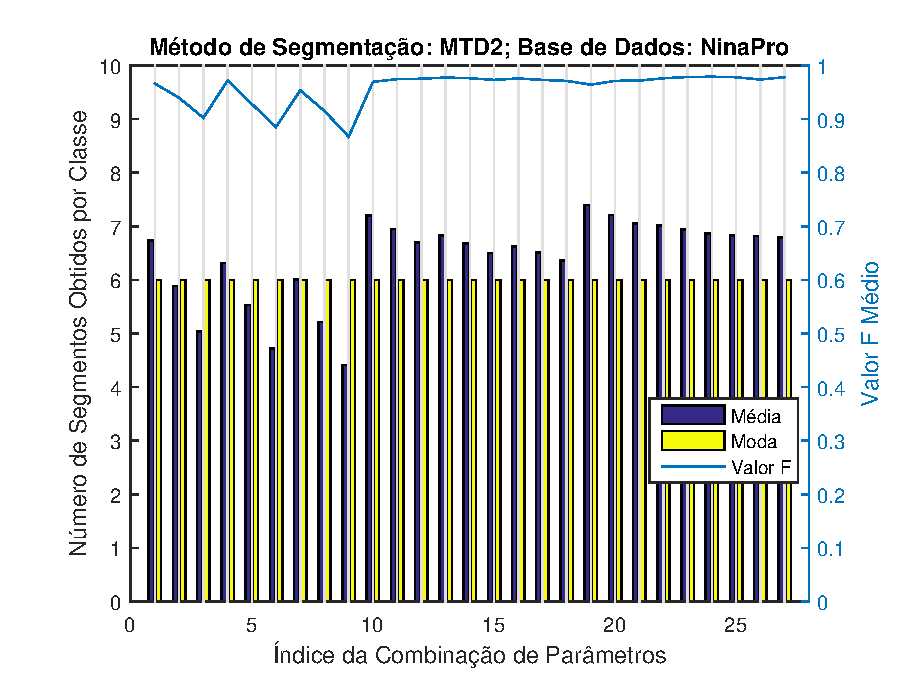
\includegraphics[width=0.8\textwidth]{./img/mtd2_nina.eps}
				\end{center}
			\end{figure}
			\begin{figure}
				\begin{center}
					\includegraphics[width=0.8\textwidth]{./img/mtd2_iee.eps}
				\end{center}
			\end{figure}
			
		\end{columns}
	\end{frame}
	
	\begin{frame}
		\frametitle{Testes com Diferentes Combinações de Parâmetros}
		\framesubtitle{MTD3 e MTD4}
		\begin{columns}[c]
		
		\column{.5\textwidth}
			\begin{figure}
				\begin{center}
					\includegraphics[width=0.8\textwidth]{./img/mtd3_nina.eps}
				\end{center}
			\end{figure}
			\begin{figure}
				\begin{center}
					\includegraphics[width=0.8\textwidth]{./img/mtd3_iee.eps}
				\end{center}
			\end{figure}
			
		\column{.5\textwidth}
			\begin{figure}
				\begin{center}
					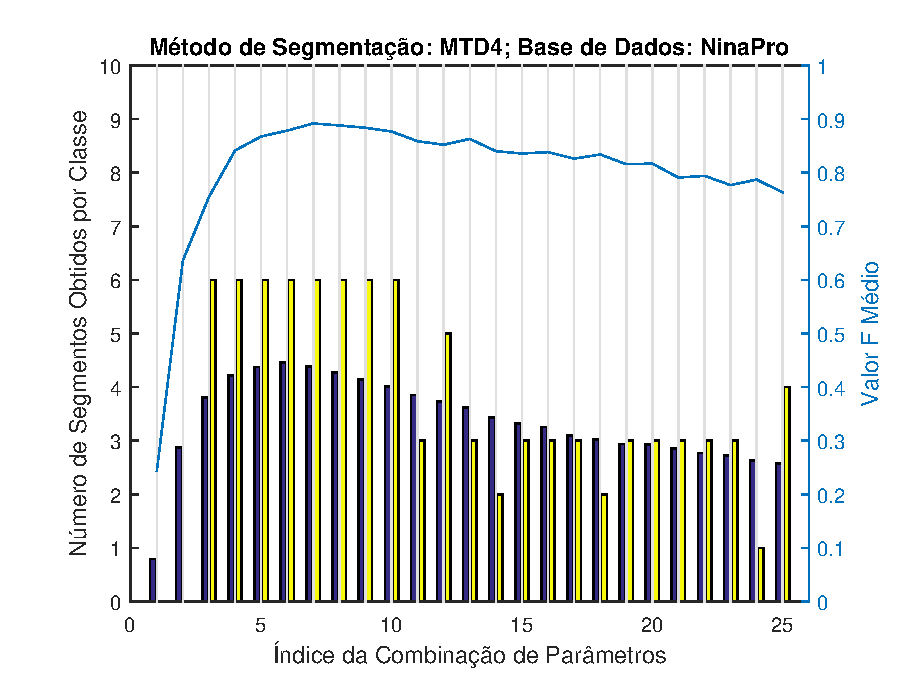
\includegraphics[width=0.8\textwidth]{./img/mtd4_nina.eps}
				\end{center}
			\end{figure}
			\begin{figure}
				\begin{center}
					\includegraphics[width=0.8\textwidth]{./img/mtd4_iee.eps}
				\end{center}
			\end{figure}
			
		\end{columns}
	\end{frame}
	
	\begin{frame}
		\frametitle{Parâmetros Selecionados}
		\framesubtitle{Combinações de parâmetros de cada método com média de número de segmentos obtidos por classe mais próximo de 6}
		
		\begin{figure}
			\begin{center}
				\includegraphics[width=\textwidth]{./img/tabelaParams.png}
			\end{center}
		\end{figure}

	\end{frame}
	
	\subsection[Resultados Utilizando Parâmetros Selecionados]{Resultados Utilizando Parâmetros Selecionados}
	
	\begin{frame}
		\frametitle{Resultados Utilizando Parâmetros Selecionados}
		\framesubtitle{Valor F por Classe de Movimento, Base de Dados NinaPro}
		
		\begin{figure}
			\begin{center}
				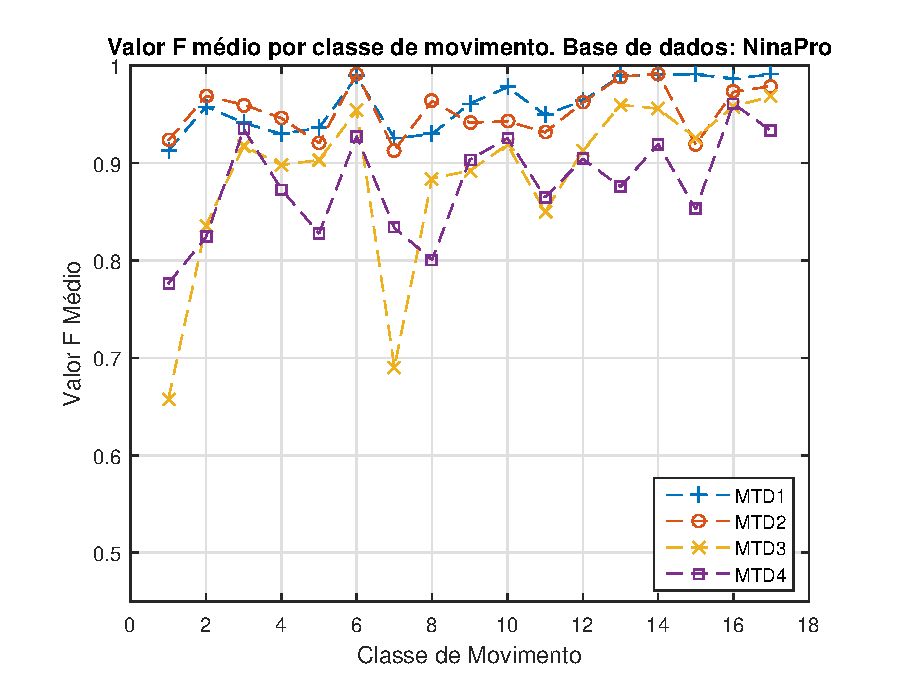
\includegraphics[width=\textwidth]{./img/fvalue_nina.eps}
			\end{center}
		\end{figure}
		
	\end{frame}
	
	\begin{frame}
		\frametitle{Resultados Utilizando Parâmetros Selecionados}
		\framesubtitle{Valor F por Classe de Movimento, Base de Dados IEE}
		
		\begin{figure}
			\begin{center}
				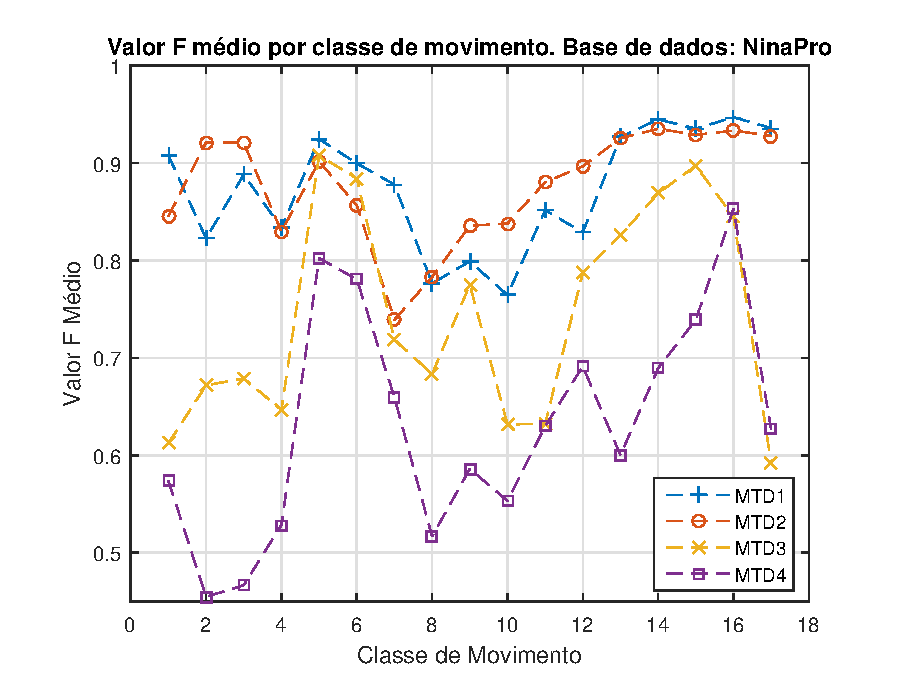
\includegraphics[width=\textwidth]{./img/fvalue_iee.eps}
			\end{center}
		\end{figure}
		
	\end{frame}
	
	\section[Conclusões]{Conclusões}

	\begin{frame}
		\frametitle{Conclusões}
		
		\begin{block}{MTD1 e MTD2 obtiveram valores F médio cerca de 17\% maiores que MTD3 e MTD4}
			\begin{itemize}
				\item Valores F de classificação similares com MTD1 e MTD2
				\item Com MTD3 e MTD4 não foi possível obter moda 6 de número de segmentos na base IEE
			\end{itemize}
		\end{block}
		
		\begin{columns}[c]
		
		\column{.5\textwidth}
		\begin{exampleblock}{Maiores Valor F médio (NinaPro): 0,96}
			\begin{itemize}
				\item 6 (flexão de todos os dedos ao punho)
				\item 14 (extensão de punho)
				\item 16 (desvio ulnar do punho)
				\item 17 (extensão de punho com mão cerrada)
			\end{itemize}
		\end{exampleblock}
		
		\column{.5\textwidth}
		\begin{alertblock}{Menores Valor F médio (NinaPro)}
			\begin{itemize}
				\item 1 (polegar esticado, flexão dos outros dedos): 0,81
				\item 7 (extensão do indicador em movimento de ``apontar''): 0,84
			\end{itemize}
		\end{alertblock}
		
		\end{columns}
	\end{frame}
		
	\begin{frame}
		Obrigado!
	\end{frame}

\end{document}